\documentclass{article}
\usepackage[%
    left=0.5in,%
    right=0.5in,%
    top=0.5in,%
    bottom=0.5in,%
]{geometry}%
\usepackage{minitoc}
\usepackage{multicol}
\usepackage{graphicx}
\usepackage{fixltx2e}
\usepackage{hyperref}
\usepackage{hyperref}
    \hypersetup{ colorlinks = true, linkcolor = blue }
\usepackage{blindtext}

\graphicspath{ {./} }

\newcommand{\inlinecode}[2]{\colorbox{lightgray}{\lstinline
[language=#1]$#2$}}
\newcommand{\worddef}[1]{\hyperref[sec:reference]{\textit{#1}}}

\begin{document}

\section{File systems}
\begin{flushleft}
A \worddef{user view} that defines a file system in terms of the abstractions that the operating system provides.
An \textbf{implementation view} that defines the file system in terms of its \textbf{low level implementation}
\end{flushleft}

\subsection{User view}
\begin{flushleft}
Important aspects of the user view include:
\begin{itemize}
	\item The file \textbf{abstraction} which hides away \textbf{implementation details} to the user (similar to processes and memory) 
	\item \textbf{File naming} policies (abstracts storage details), “user file attributes” (e.g. size, protection, owner, protection, dates)
	\item There are also \textbf{system attributes} for files (e.g. non-human readable file descriptors (similar to a PID), archive flag, temporary flag, etc.)
	\item Directory structures and organisation
	\item System calls to interact with the file system
\end{itemize}
\end{flushleft}

\subsection{Structures}
\subsubsection{Overview}
\begin{flushleft}
Different directory structures have been used over the years
\begin{itemize}
	\item Single level: all files in the same directory (reborn in consumer electronics)
	\item Two or multiple level directories (hierarchical): tree structures
	\item Absolute path name: from the root of the file system Relative path name: the current working directory is used as the starting point
	\item Directed acyclic graph (DAG): allows files to be shared (i.e. links to files or sub-directories) but cycles are forbidden
	\item Generic graph structure in which links and \textbf{cycles can exist}
\end{itemize}
The use of \textbf{DAGs} and \textbf{generic graph} structures results in significant complications in the implementation
\end{flushleft}

\subsubsection{DAG and graph complications}
\begin{flushleft}
When searching the file system:
\begin{itemize}
	\item Cycles can result in \textbf{infinite loops}.
	\item Sub-trees can be traversed \textbf{multiple times}.
\end{itemize}
Files have \textbf{multiple} absolute file names. Deleting files becomes a lot more \textbf{complicated} (i.e. links may no longer point to a file, \textbf{inaccessible cycles} may exist). A \textit{garbage collection} scheme may be required to remove files that are \textbf{no longer accessible} from the file system tree (that are part of a cycle only)
\end{flushleft}

\subsection{Directories}
\begin{flushleft}
Directories contain a list of \textbf{human readable} file names that are mapped onto unique identifiers and disk locations. They provide a \textbf{mapping} of the \textbf{logical} file onto the \textbf{physical} location. Retrieving a file comes down to searching a directory file as fast as possible: 
\begin{itemize}
	\item A simple random order of directory entries might be \textbf{insufficient} (search time is linear as a function of the number of entries)
	\item Indexes or \textit{hash tables} can be used
	\item They can store all file related attributes (e.g. file name, disk address – Windows) or they can contain a \textbf{pointer} to the data structure that \textbf{contains} the details of the file (Unix)
\end{itemize}
\end{flushleft}

\subsubsection{System calls}
\begin{flushleft}
Similar to files, directories are manipulated using system calls: 
\begin{itemize}
	\item create/delete: a new directory is created/deleted
	\item opendir, closedir: add/free directory to/from internal tables
	\item readdir, return the next entry in the directory file
	\item Others: rename, link, unlink, list, update 
\end{itemize}
Directories are special \textbf{files} that \textbf{group files} together and of which the structure is defined by the file system. \textbf{A bit is set to indicate that they are directories}!
\end{flushleft}


\section{Files}
\subsection{Types}
\begin{flushleft}
Many OSs support \textbf{several} types of file. Both Windows and Unix (including OS X) have regular files and directories:
\begin{itemize}
	\item Regular files contain user data in ASCII or binary (well defined) format
	\item Directories group files together (but are files on an implementation level)
\end{itemize}
Unix also has character and block special files:
\begin{itemize}
	\item \textbf{Character} special files are used to model \textbf{serial I/O devices} (e.g. keyboards, printers)
	\item \textbf{Block} special files are used to model, e.g. \textbf{hard drives}
\end{itemize}
\end{flushleft}

\section{System calls}
\subsection{Types}
\begin{flushleft}
File control blocks (\textbf{FCBs}) are kernel data structures, i.e. they are \textbf{protected} and only accessible in \textit{kernel mode}! Allowing user applications to access them directly could \textbf{compromise} their integrity System calls enable a user application to \textbf{ask} the operating system to carry out an action on its behalf (in kernel mode).\\
There are two different categories of system calls:
\begin{itemize}
	\item File manipulation: \texttt{open(), close(), read(), write(), ...}
	\item Directory manipulation: \texttt{create(), delete(), readdir(), rename(), link(), unlink(), list(), update()}
\end{itemize}
\end{flushleft}

\section{Implementation context}
\begin{flushleft}
Irrespectively of the type of file system, a number of \textbf{additional} considerations have to be addressed, including:
\begin{itemize}
	\item Disk partitions, partition tables, boot sectors, etc.
	\item Free space management (free memory)
	\item System wide and per process file tables (process tables)
\end{itemize}
Low level formatting \textbf{writes} sectors to the disk, high level formatting \textbf{imposes a file system} on top of this (using blocks that can can cover multiple sectors).
\end{flushleft}

\section{Hard Disk Structures}
\begin{flushleft}
Disks are usually \textbf{divided} into multiple partitions. An \textbf{independent} file system may exist on each partition. \textbf{Master boot record} is located at start of the entire drive:
\begin{itemize}
	\item Used to \textbf{boot} the computer (BIOS reads and executes MBR)
	\item Contains \textit{partition table} at its end with active partition
	\item One partition is listed as \textbf{active} containing a boot block to \textbf{load the operating system}
\end{itemize}
\end{flushleft}
\begin{center}
	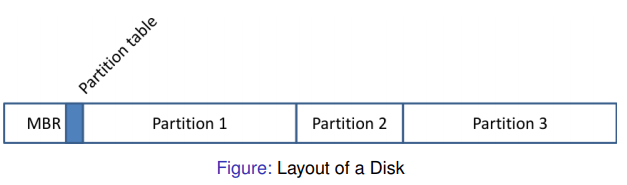
\includegraphics[scale=0.4]{disk_partition.png}
\end{center}

\section{Partition layouts}
\begin{flushleft}
The layout of a partition differs depending on the file system A UNIX partition contains:
\begin{itemize}
	\item  The partition boot block: Contains \textbf{code to boot} the operating system. \textbf{Every} partition has boot block – \textbf{even if} it does not contain OS
	\item Super block contains the \textbf{partition’s details}, e.g., partition size, number of blocks, I-node table size
	\item Free space management contains, e.g., a bitmap or linked list that indicates the free blocks
	\item I-nodes: an array of data structures, one per file, telling all about the files
	\item Root directory: the top of the file-system tree
	\item Data: files and directories
\end{itemize}
\end{flushleft}
\begin{center}
	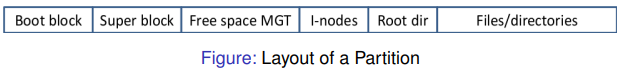
\includegraphics[scale=0.5]{partition_layout.png}
\end{center}

\section{Disk space management}
\begin{flushleft}
Two methods are commonly used to keep track of free disk space: \textit{bitmaps} and \textit{linked lists}. Note that these approaches are very similar to the ones to keep track of \textbf{free memory}.
\begin{itemize}
	\item Bitmaps represent each block by a \textbf{single bit} in a map 
	\item The size of the bitmap \textbf{grows with the size} of the disk but is \textbf{constant} for a given disk
	\item Bitmaps take comparably \textbf{less space} than linked lists
\end{itemize}
A Linked List of disk blocks (also known as \textbf{Grouping}).
\begin{itemize}
	\item We use \textbf{free blocks} to hold the \textbf{numbers of the free blocks} (hence, they are no longer free). E.g. with a 1KB block a 32-bit disk block number, each block will hold 255 free blocks (one for the pointer to the next block). Since the free list \textbf{shrinks} when the disk becomes full, this \textbf{is not wasted space}.
	\item Blocks are linked together, i.e., multiple blocks list the free blocks
	\item The size of the list \textbf{grows} with the size of the disk and \textbf{shrinks} with the size of the blocks
	\item Linked lists can be modified by keeping track of the number of \textbf{consecutive free blocks} for each entry (known as Counting)
\end{itemize}
\end{flushleft}

\subsection{Comparison}
\begin{flushleft}
\textbf{Bitmaps:}
\begin{itemize}
	\item  Require extra space. E.g: If block size = 212 bytes and disk size = 230 bytes (1 GB) ⇒ bitmap size: 230/2 12 = 218 (32KB)
	\item Keeping it in main memory is possible only for \textbf{small disks}. 
\end{itemize}
\textbf{Linked lists:}
\begin{itemize}
	\item \textbf{No waste} of disk space
	\item We only need to keep in memory \textbf{one block} of pointers (load a new block when need)
\end{itemize}
\end{flushleft}

\section{File tables}
\begin{flushleft}
Apart from the free space memory tables, there is a number of key data structures stored in memory: 
\begin{itemize}
	\item An in-memory mount table
	\item An in-memory directory cache of \textbf{recently} accessed directory information
	\item A \textbf{system-wide} open file table, containing a copy of the FCB for every currently open file in the system, including location on disk, file size, and “open count’ (number of processes that use the file)
	\item A \textbf{per-process} open file table, containing a pointer to the system open file table
\end{itemize}
\end{flushleft}

\pagebreak
\section*{Reference section} \label{sec:reference}
\begin{description}
	\item[user view] \hfill \\ The user view defines how the file system looks like to regular users
(and programmers) and relates to abstractions
\end{description}
\end{document}
